%%%%%%%%%%%%%%%%%%%%%%%%%%%
\chapter {Parallel Black Virus Decontamination in Arbitrary Graph}
\label{TL}
%%%%%%%%%%%%%%%%%%%%%%%%%%%

\section{Introduction}
In \cite{Cai}, he proposes two exploration strategies: Greedy Exploration and Threshold Exploration, both spread optimal and total number of agents asymptotical optimal. Since these strategies are sequential, they are time consuming($O(\Delta n^2)$).  In order to explore the graph parallelly, we propose two different strategies: \\
(1) Flood Strategy\\
(2) Castle First Strategy\\
The general idea of the Flood Strategy is simple, supposing that an agent resides in node $v$, and it has $i$ neighbours excepted to be explored, then it simply clones $v$ agents and send them to its neighbours. In Castle First Strategy, we build castles which is a node or the combination of several nodes(rules are introduced later), the exploration phase can be viewed as the combination of many smaller scale exploration in the graph which begins with the location of one of the exploring group and ends with one of the unexplored castles. After all the castles are explored, all the nodes in the graph are explored. The general exploring strategy for these two strategies is based on the one described in Chapter 3 which consists of performing a {\em Shadowed Exploration} phase to locate the BV, followed by a {\em Surrounding and Elimination} phase to eliminate the cloned BVs. 

Strategy {\em Flood}  is time optimal with the cost of a great number of agents while strategy {\em Castle First} comes to a compromise between the strategy {\em Flood} and the sequential strategies: it employ much less agents than the strategy {\em Flood} while cost much less time than the sequential strategies. 

In the arbitrary graph, we assume that any node does not disconnect the graph.

\section{Parallel Strategies for BV Decontamination in Arbitrary Graph}
\subsection{Flood Strategy}
\noindent{\bf Initialization}
In this strategy, all the agents are endowed with 3-hop visibility. Also, all the agents do not need to remember the routes they pass. Finally, in this strategy, we use an important ability of agents which is clone. As we introduced in Chapter 2, clone means that a agent is endowed with the capacity to generate one or more agent. 

We use the Dijkstra Algorithm to compute the shortest route step for every node and write them on the white board on each node, so for each node, there should be a number (Shortest Route Number) recording the number of steps of the shortest route from the homebase to it. Let us denote by $v_{SRN}$ the Shortest Route Number of node $v$, and nodes ${v_1, \ldots, v_i}$ are neighbours of node $v$ assuming that $v$ has $i$ neighbours. Then edges connecting node $v$ and its neighbours are $e(v, v_1), \ldots, e(v, v_i)$. We write the $v_{SRN}$ to the end of these edges (the end connecting to its neighbours), so when an agent resides in any node from $v_1$ to $v_i$, it can see the Shortest Route Number of node v because of the local visibility. (For example, see Fig\ref{fig:Arbi1}) 

\begin{figure}[H]
  \centering  
  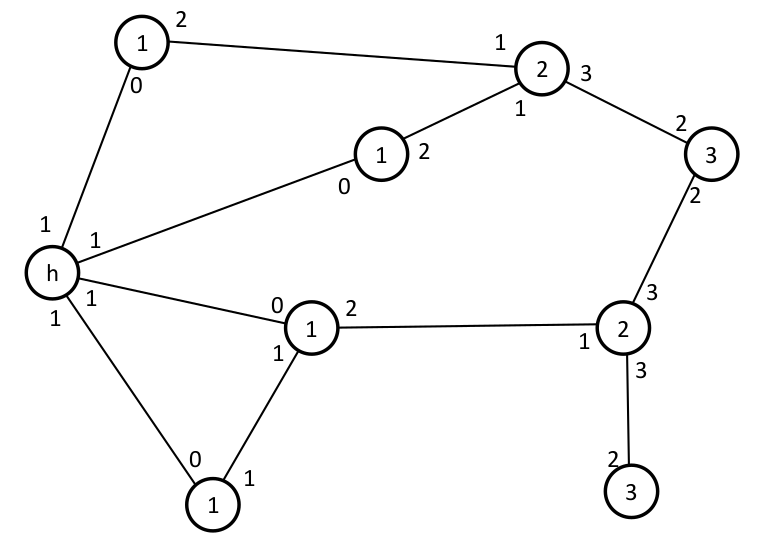
\includegraphics[width=3in]{figures/Arbi1.png}
  \caption{Initialization of the graph}\label{fig:Arbi1}
\end{figure}

\noindent{\bf Exploration Phase}
All the agents in this strategy follow the same rules in the exploration phase.

Rules for agents in the exploration phase:
Let us denote by $SNR$ the Shortest Route Number.
\begin{enumerate}
\item Agents can only move from node with lower $SNR$ to node with higher $SNR$.
\item Assuming that there are $x$ agents residing in node $v$, and the next destination(s) are $\{v_1,\ldots, v_i\}$. 

        if $x\geq i+1$, then $i$ agents move to the destinations respectively while one agent stays in node $v$ to guard $v$ at $T_i$. If one of agents is destroyed, the Elimination phase begins; if none of the agents is destroyed, the left $x-(i+1)+1(the one who guards the node $v$)$ agents evenly move to the destinations at $T_{i+1}$. 
        if $x< i+1$, then one of the agents residing in node $v$ clones $i+1-x$ agents, and these $i$ agents move to all the neighbours at $T_i$. If one of the agents is destroyed, the Elimination phase begins; if none of the agents is destroyed, the agent guarding the node $v$ randomly moves to one neighbour with $SNR$ equal to $a+1$ at $T_{i+1}$.
\item If an agent resides in a node (assuming its $SNR$ is $a$) without any neighbour whose $SNR$ equal to $a+1$, then it simply stays there.
 
        Since all the action of agents happen after they meet each other at the same node, they can communicate with each other and make sure that all their routes do not conflict.
\end{enumerate}
An example of how the agents move is showed in Fig\ref{fig:Arbiflood}
\begin{figure} [H]
  \centering 
  \subfigure[$T_1$]{ 
    \label{fig:Arbiflood1:a} %% label for first subfigure 
    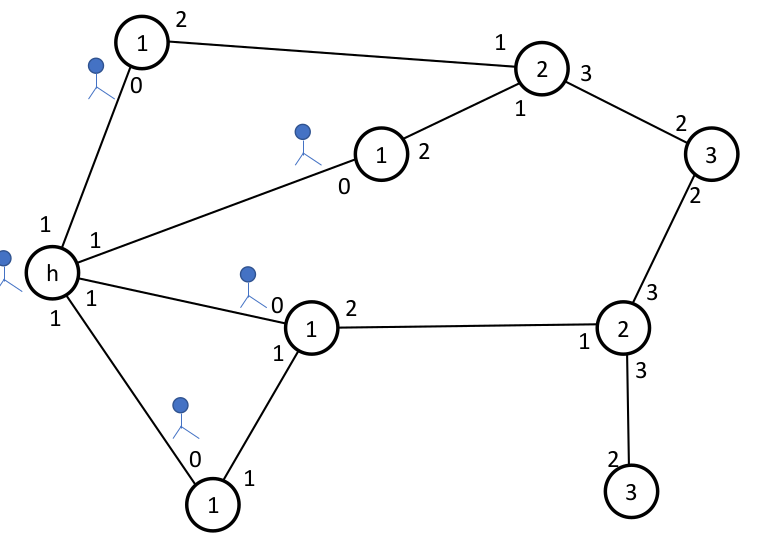
\includegraphics[width=2.5in]{figures/Arbiflood1.png}} 
%  \hspace{1in} 
  \subfigure[$T_2$]{ 
    \label{fig:Arbiflood2:b} %% label for second subfigure 
    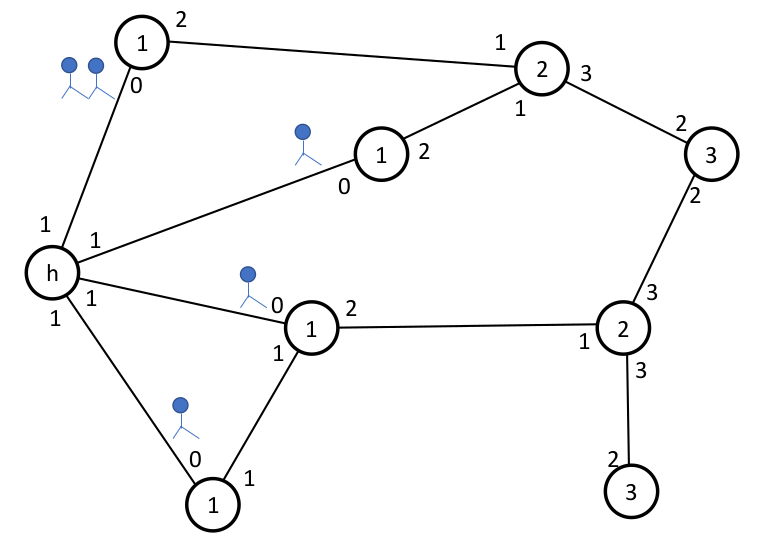
\includegraphics[width=2.5in]{figures/Arbiflood2.png}}
    \hspace{1in} 
  \subfigure[$T_3$]{ 
    \label{fig:Arbiflood3:c} %% label for second subfigure 
    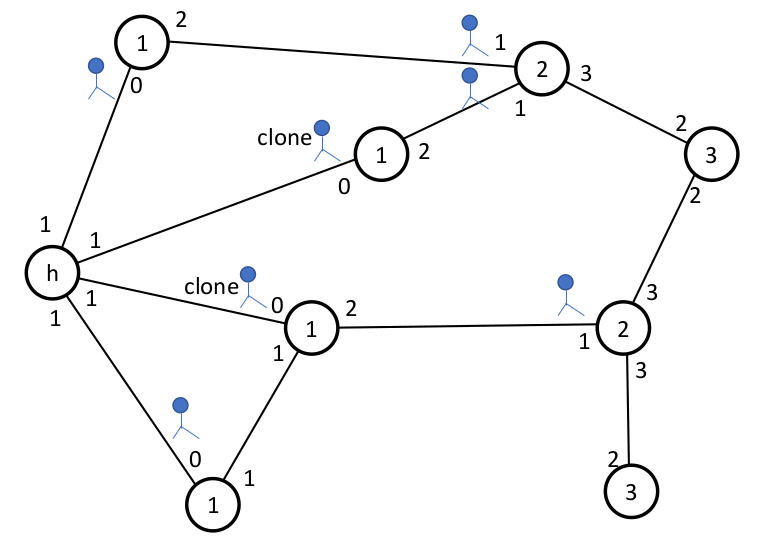
\includegraphics[width=2.5in]{figures/Arbiflood3.png}}
%      \hspace{1in} 
  \subfigure[$T_4$]{ 
    \label{fig:Arbiflood4:d} %% label for second subfigure 
    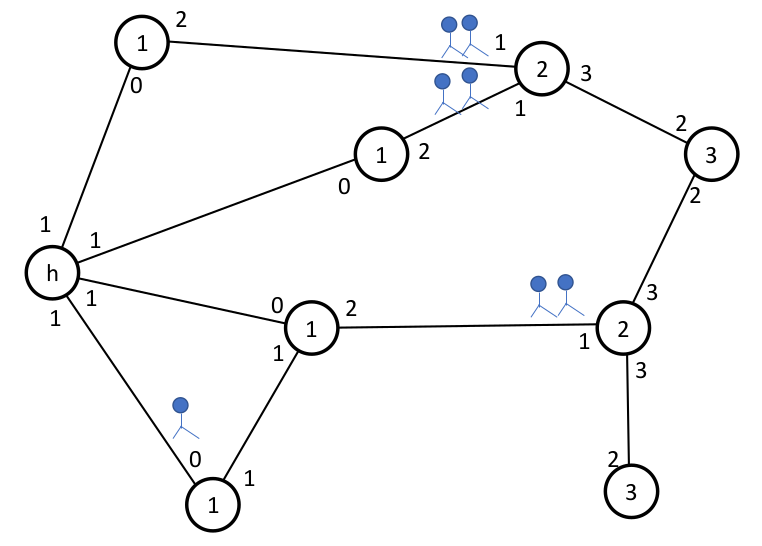
\includegraphics[width=2.5in]{figures/Arbiflood4.png}}
      \hspace{1in} 
  \subfigure[$T_5$]{ 
    \label{fig:Arbiflood5:e} %% label for second subfigure 
    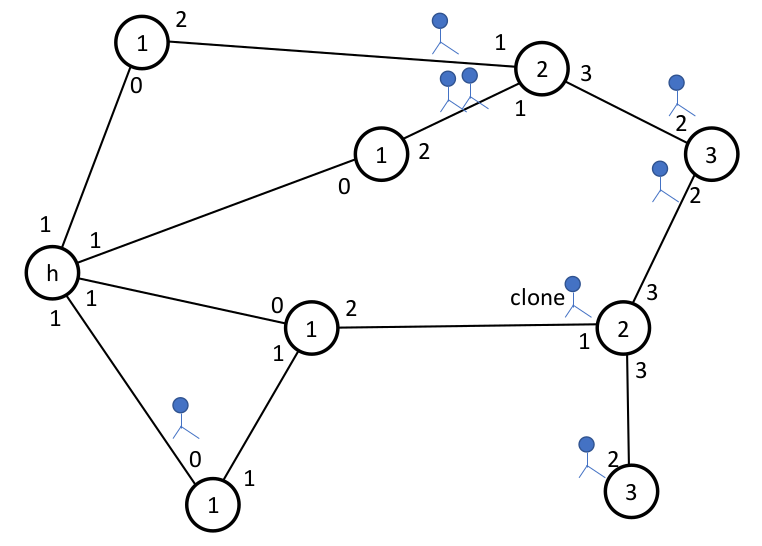
\includegraphics[width=2.5in]{figures/Arbiflood5.png}}
     \subfigure[$T_6$]{ 
    \label{fig:Arbiflood6:e} %% label for second subfigure 
    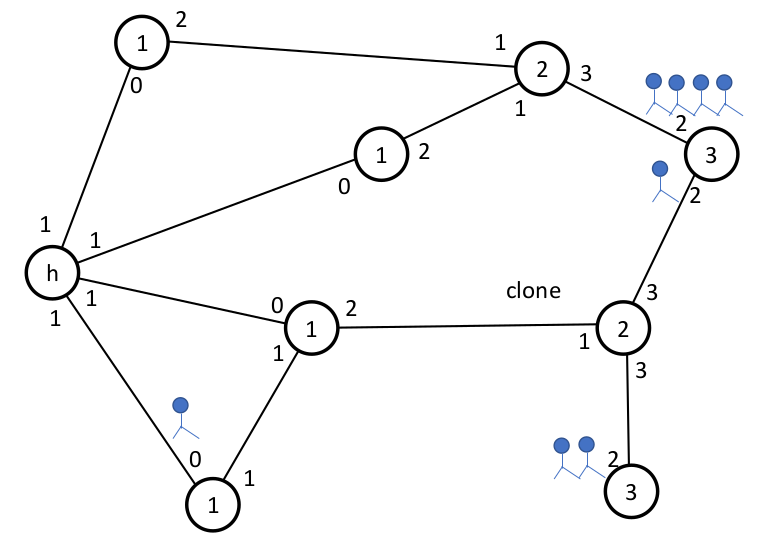
\includegraphics[width=2.5in]{figures/Arbiflood6.png}}
  \caption{An example of how the agents move in the Flood Strategy} 
  \label{fig:Arbiflood} %% label for entire figure 
\end{figure}

\noindent{\bf Elimination Phase}
Let us assume that the node where the original BV resides is $v$ with $SNR$ equal to $a$ and it is triggered at $T_i$. Then at this time, the clones spread to all neighbours of node $v$ with $SNR$ equal to $a+1$ and survive while leaving node $v$ clean (no agent and no BV) and let us denote by $v_{BV}$s all these BV nodes.  

Now we introduce how agents residing in different positions move in the Elimination phase.
\begin{enumerate}

\item Rule 1: We call agents residing in the these $v_{BV}$s' neighbours with $SNR$ equal to $a$ the Witness Agent, and these Witness Agent can easily realize whether or not node $v$ is the place where the original BV resides. For example, since they have 3-hop visibility, so if they see that one of their ``2-distance" neighbours (say node $v'$) does not contains an agent but some neighbours of node $v'$ contain agents, then they can know that the original BV resides in node $v$. If the Witness Agents realize the existence of BV at $T_1$, then they simply stop cloning and moving. 

\item Rule 2: For all of the agents residing in node $v$'s neighbours with $SNR$ equal to $a-1$ (say the number of them is $y$), they receive clones and realize the location of the BV and would move to $v$ at $T_{i+1}$. Let us denote by $z$ the number of $v$'s neighbours with $SNR$ equal to $a+1$, then if $y< z+1$, one of the agents residing in node $v$ should clone another $z+1-y$ agents and then $z$ agents move to $v$'s neighbours with $SNR$ equal to $a+1$ at $T_{i+2}$.
\end{enumerate}

See Fig\ref{fig:Arbiflood}. For convenience of description, we give every node in the graph a distinct ID from 1 to 13. As shown in the picture, when the BV is triggered, the clones spread to all neighbours of node 3, and node 4 and 5 become new BV node while nodes 1, 2 and 12 destroy a clone respectively and realize that the original BV resides in node 3.

\begin{figure}[H]
  \centering  
  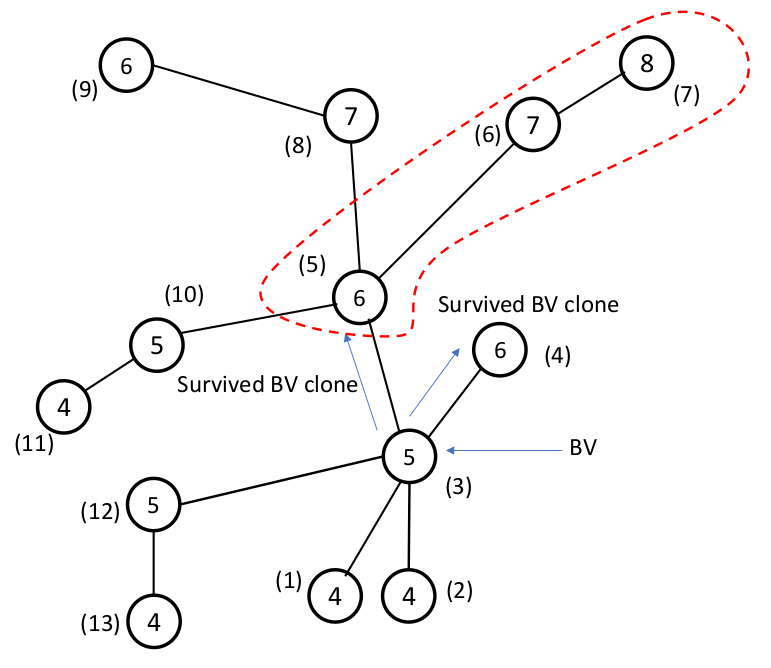
\includegraphics[width=3in]{figures/Arbi3.png}
  \caption{An possible situation when the BV is detected}\label{fig:Arbi3}
\end{figure} 

In Fig.\ref{fig:Arbi3}, node 10 is a Witness Agent and because of the 3-hop visibility, it can ``see" that there is no agent residing in node 3 but there are agents residing in node 3's neighbours which are node 1 and node 2. By this way, it knows that the original BV resides in node 3 and it stop moving and cloning.

For convenience, let us denote by $a$ the $SNR$ of the original BV node. Since in our assumption, any node does not disconnect the graph, so the following situation would not happen:
\begin{enumerate}
\item All the higher $SNR$ neighbours of the new formed BVs have only one neighbour with lower $SNR$ and it is the BV node, \item Some of the neighbours of the new formed BVs have at least one neighbour with lower $SNR$ except their BV neighbour while some of the neighbours of the new formed BVs have only one neighbour with lower $SNR$.
\end{enumerate}
For example, see \ref{fig:Arbi3}. The situation shown in the red circle is the case when the node 5 disconnect the graph.The new formed BVs has two higher $SNR$ neighbours which are nodes 8 and 6. Node 6 has only one neighbour with lower $SNR$ and it is the BV node. Assuming the BV is triggered at $T_i$, then at $T_{i+2}$, all the BVs are decontaminated except one: the BV clone spreading to node 6, so we can only employ an agent to move to node 6, then to node 7 and the BV is permanently destroyed and we do not want it to happen.

With our assumption, all the higher $SNR$ neighbours of the new formed BVs have at least one neighbour with lower $SNR$ except their BV neighbour.  Since agents who do not know the existence of the BV keep moving and at $T_{i+2}$, they would move to occupy nodes with $SNR$ equal to 7 which means all the neighbours of the new formed BV are guarded. In this way, all the BVs are permanently destroyed at $T_{i+2}$.

               
\subsection{Castle First Strategy}
\noindent{\bf Introduction}
In the Castle First Strategy, all the agents have only the local visibility. But the leader agent in each exploration group have the map of the graph in its memory. Also, the leader agents are endowed with the ability of clone.

In the Castle First Strategy, we built some castles based on the graph with $SNR$. More than one group of agents are sent to explore the graph respectively. Their exploration of the graph are separated into many ``sub-exploration"s and each ``sub-exploration" begins with where the agents are and ends with a new unexplored castle. The map of the graph with all the castles being pointing out is recorded on the whiteboard on nodes with more than two neighbours (the intersection) so when agents move across these nodes, they can update the information on the whiteboard (for example, changing the state of some castles into explored) or update its own memory. When agents cannot find an unexplored castle in the graph, then they terminate. 

\noindent{\bf Initialization}
Based on the graph marked $SNR$ for every node, we built another graph called ``Castle Graph". 
We now give the definition of ``Castle":
\begin{enumerate}
\item Case 1: Node who has one neighbour is a ``Castle".
\item Case 2: If a node has at least one neighbour with the same $SNR$ as it, then the combination of them is a castle. If different castles have at least one common node, then we merge them into a bigger castle;
\item Case 3: If a node has more than two neighbours with lower $SNR$ than itself, than this node is a castle.
\end{enumerate}

Some examples of castles are shown in Fig\ref{fig:CastleExample}
\begin{figure}[H]
  \centering  
  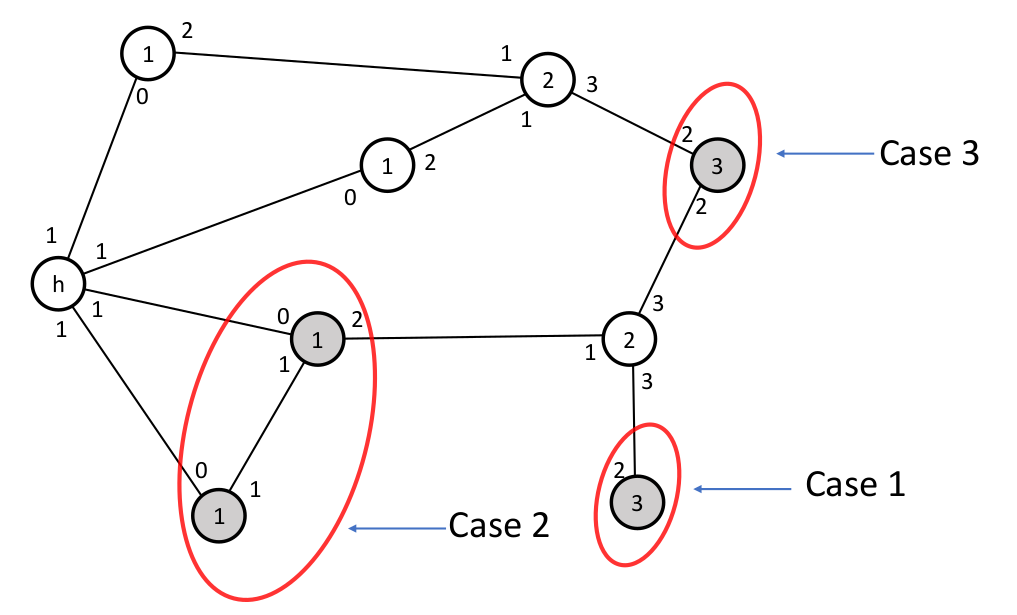
\includegraphics[width=3.5in]{figures/CastleExample.png}
  \caption{Examples of Castles}\label{fig:CastleExample}
\end{figure} 

After the processing, we have a new graph called ``Castle Graph" and this graph is presented on the whiteboard on the nodes which have more than two neighbours, so when the agent reach this node, it can read the graph to update its own information or using its own information to update the ``Castle Graph". 

\noindent{\bf Exploration Phase}
There are two principle in the exploration phase for the agents:
\begin{enumerate}
\item when agents move in an unexplored area, they should strictly move from node with smaller $SNR$ to node with bigger $SNR$ and should follow the ``casual walk" while when move in an explored area, they can move in opposite (from bigger $SNR$ to smaller $SNR$) and when the agents move in this area, they are allowed not to follow the ``casual walk" (for example, when they plan to explore node $v$ from node $u$, the LA can directly move to node $v$ when node $v$ is in the explored area) which is called ``normal walk".
\item The castle selected to be the destination of the ``sub exploration" should meet the follow the following requirement: assuming that the $SNR$ of the destination castle is $a$ and the node from where the agents start the ``sub exploration" is $v$  , then for every node with $SNR$ equal to $a-1$ connected to the castle, there should be a route from $v$ to these nodes and no castle(s) which are not explored (the castles can be in the state of ``under exploring" or ``explored") existing on these routes. In another word, when the agents move from $v$ to these node, except the destination castle, they do not need to ``attack" other castles. 
\end{enumerate}  

There are two kind of agents in this strategy: Leader Agent (LA) and Shadow Agent(SA) and the LA has the map of the whole graph in its mind. When more agents are needed, the LA would clone the agents. At the beginning of the exploration phase, the LAs are in the homebase, so they respectively pick a castle to be the destination of the their first ``sub exploration" and since they have the map of the graph, they can compute a shortest route for the ``sub exploration" and then are sent randomly from the homebase. 

The agents are divided into three status: Finding Castle, Attacking Castle and Waiting in Line. 

Initially, the status of all agent group are ``Finding Castle".In a agent group with the status of ``Finding Castle", if the LA in that agent group can find an available castle, then the status of this group changes into ``Attacking castle". Unless the agent group realizing the existence of BV, the status of the agent group changes into ``Finding Castle" at the end; if the LA in that agent group cannot find an available castle but there are still castle unexplored in the group, then the status of this group changes into ``Waiting in line". Unless the agent group realizing the existence of BV, the status of agent group changes into ``Finding Castle" at the end. 

When the status of an agent group changes into ``Attacking Castle", the LA in this exploring group updates the information on the whiteboard on the node along its route to that castle. On the way to their destination (the castle), the agents follow the ``casual walk" in the unexplored area and ``normal walk" in the explored area: when exploring the node $u$ from the node $v$, one of the SAs moves to node $u$, when the node $u$ is safe, it returns to node $v$ and moves to the node $u$ with the LA and the other SAs; when the node $u$ contains a BV, then the LA knows the existence of the BV by receiving the clone of the BV.   

Along the route to the group's destination, the LA updates the information (changing the state of the destination castle to be under explored) of the intersections and also read information from them, if it finds that the destination castle of its ``sub exploration" has been explored or under exploring (for example, when it read the information from the whiteboard of the intersection on the route and it shows that that destination castle's state is ``explored" or ``under exploring"), then the status of its group changes into ``Finding Castle" again. If not, then this group reach one of the destination castle's lower $SNR$ neighbour and the LA starts to arrange the SAs to guard all the lower $SNR$ neighbour(s) of the castle. 

After the arrangement of the SAs, it should be ensured that all the lower $SNR$ neighbours of the castle are guarded and assuming that there are $x$ nodes in the castle $\{castle\_0, \ldots, castle\_x\}$, another $x$ SAs (Attacking Agent) should move to these $x$ nodes at the same time. In order to do that, we propose one possible strategy for the LA to place the SAs: assuming that the sequence of the nodes which should be guarded is $\{node\_0, \ldots, node\_y\}$, and $node\_i$ is the last node in the sequence connected to $castle\_k$ where $0\leq i\leq y$, $0\leq k\leq x$, then the LA should place two agents in $node\_i$ while place one agent in the other nodes when it moves in sequence to place the SAs. Also, the LA knows the time when it finishes the arrangement of the last agent(s), then it should inform the agents the exact time to move to the castle nodes and permanently destroy the BVs.

When one agent group starts to surround the castle, by which we mean that the LA has placed SAs in at least one lower $SNR$ of the castle, it is possible that another agent group has started to surround the castle (even the LA updates the information when it moves, still the consistency of all the information cannot be guaranteed). The LA of an agent group realize this by meeting an SA not from its group when it arranges the SAs to guard the lower $SNR$ neighbours of the castle. We prefer to avoid conflict when two agent group explore one castle (SAs from two different agent group move to the castle nodes). The LA can compute the time when the arrangement is finished and record it on a timestamp, so when the LA places the SAs, it leaves timestamp with these SAs. By doing this, every SA from one agent group guarding the castle hold a timestamp recording when does the arrangement end and if a LA meet a SA from other agent group with a earlier timestamp, it move back to collect the SAs in its group that have been placed and the status of this agent group turn into ``Finding Castle". 

When the arrangement is done, the LA resides in the last node needing guarded and in the next unit of time, all the Attacking Agents move to the castle nodes. Note that at this time, if there is a BV in the castle, not all the guarding agents can receive a BV clone.(see Fig\ref{fig:MultiCastleNode}
%\begin{figure}[H]
 % \centering  
 % 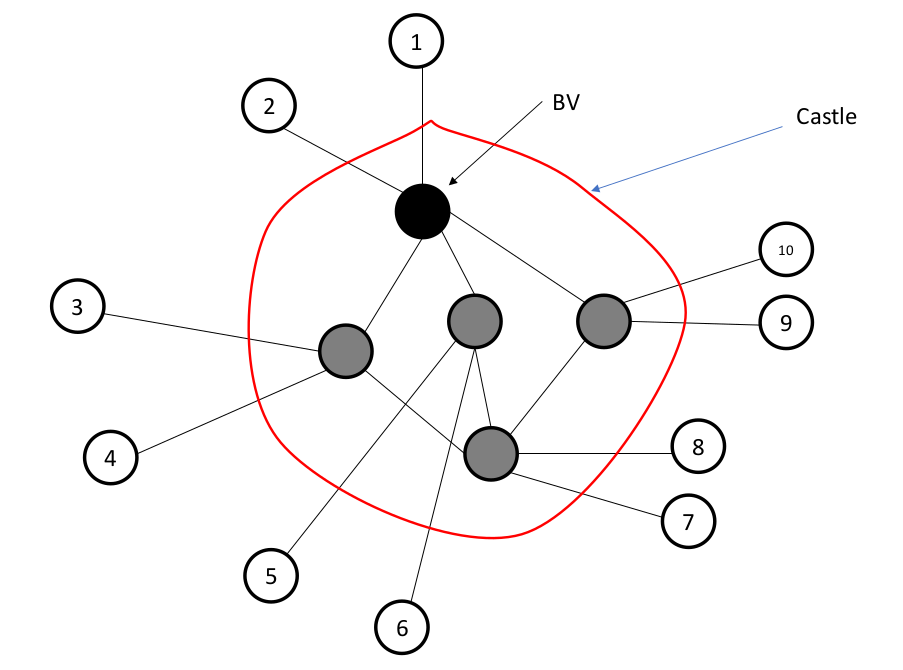
\includegraphics[width=3.5in]{figures/MultiCastleNode.png}
 % \caption{An example shows that if there is a BV in the castle, in some cases not all the guarding agents can receive a BV clone}\label{fig:MultiCastleNode}
%\end{figure} 

So after the ``attacking" by the ``Attacking agent", the LA should execute the ``Double Patrol". Now we introduce what is the ``Double Patrol".



\noindent{\bf Eliminaiotn Phase}

When the BV is triggered, then the location of the BV can be in a castle or outside the castle. In both situation, the lower $SNR$ neighbours of the BV node or the castle containing the BV have been guarded by the agents. In another word, when the BV is triggered, only the clones spreading to the higher $SNR$ neighbours (say that the number of them is $y$) survive and their locations are exposed. Also, the locations of all the neighbours of these new formed BVs are exposed. 

So the LA computes the route from where it resides to all the nodes needing guarded (guarding node). When the location of the original BV is outside the castle, then all the SAs stays with the LA, so the LA simply sends the SAs to these guarding node. When the original BV is in the castle, then the SAs are guarding the lower $SNR$ neighbours of the castle. So first all of the SAs move to the node where the original BV resides, and then the LA send the SAs to these guarding nodes. By saying sending the SAs to these guarding nodes, the LA actually tells the route to a specific destination and with the route the SA can move without the guidance of the LA. The LA knows the longest routes among these agents (say the length of it is $x$), so it wait $x+1$ unit of time after it sends the agent and send  $y$ agents to the new formed BV nodes and permanently destroy them.







 